\documentclass[11pt,a4paper]{article}
\usepackage[utf8]{inputenc}
\usepackage[english]{babel}
\usepackage[T1]{fontenc}
\usepackage{amsmath}
\usepackage{amsfonts}
\usepackage{amssymb}
\usepackage{graphicx}
\usepackage{array}
\usepackage{multirow}
\usepackage[left=2cm,right=2cm,top=2cm,bottom=2cm]{geometry}
\author{Guillem Tocabens}
\title{First measurements}
\begin{document}

\section{Theory and background} \label{theory}

\section{Scanning the prototype detector}

\subsection{Overall setup} \label{setup}

The setup uses three detectors: two scintillator detectors, placed on the sides (black squared boxes on the picture, Figure \ref{Setup}) and one semiconductor detector - hyperpure germanium detector - below the collimated source (grey cylinder on the picture). The source is placed on the top lead brick which contains a hole in the middle to collimate the radioactive source. In that position, the source is 97mm from the top of the crystal, which is 5mm from the top of the cryostat, and collimated in a 5mm hole through an 80mm lead brick. the source is covered by a little lead brick and the setup is shielded by lead to avoid propagation of gamma radiation away from the setup (see Figure \ref{Setup_front}).

\begin{figure}[!h]
\centering
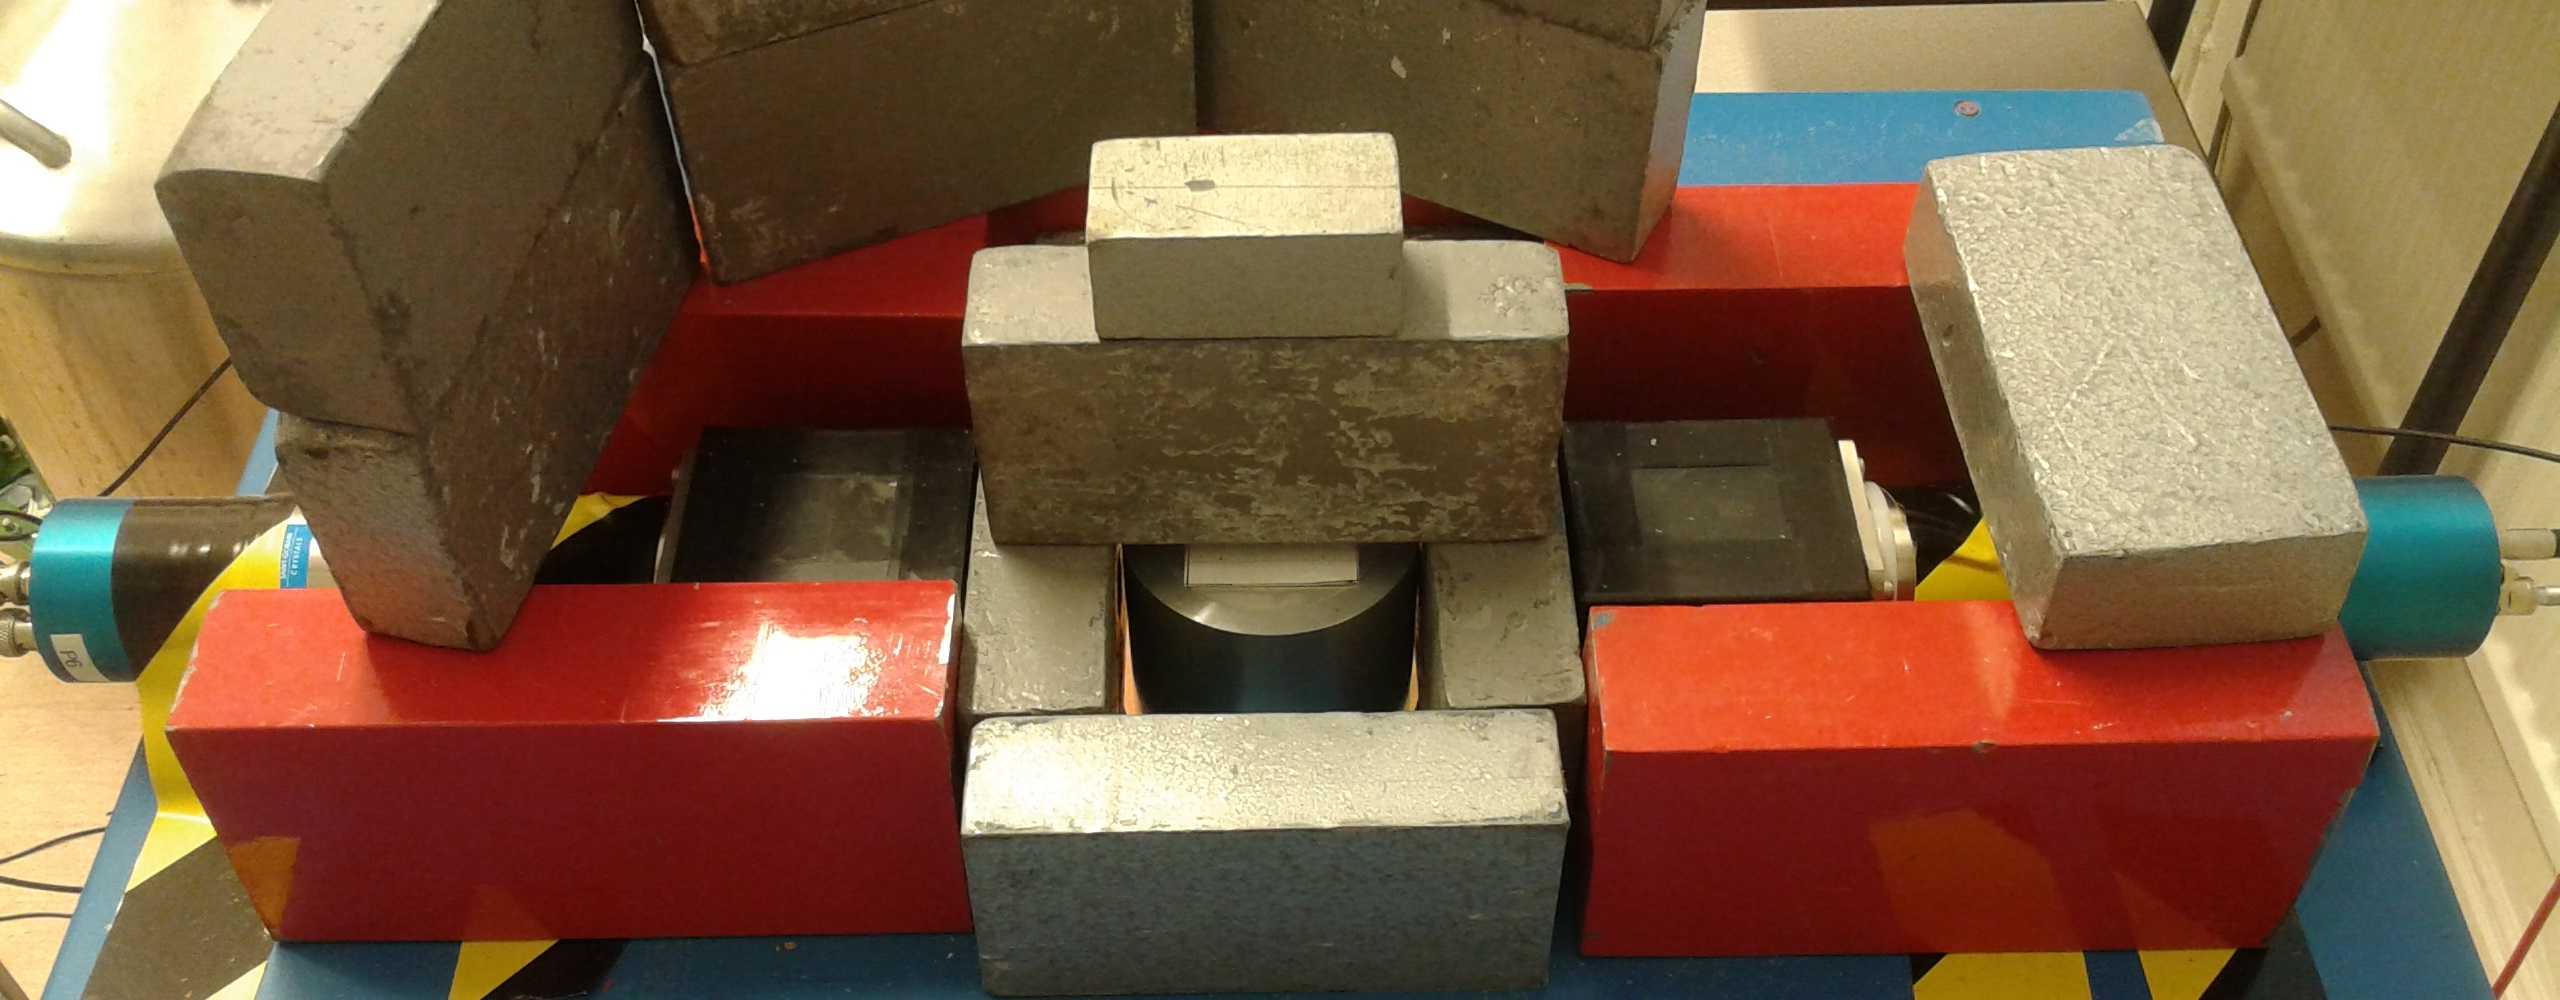
\includegraphics[scale=0.15]{New_setup_back.jpg}
\caption{Back of the original setup. The scintillator detectors are the black squared boxes on the sides of the germanium detector, placed in a cryostat (grey cylinder in the middle).}
\label{Setup}
\end{figure}

\begin{figure}[!h]
\centering
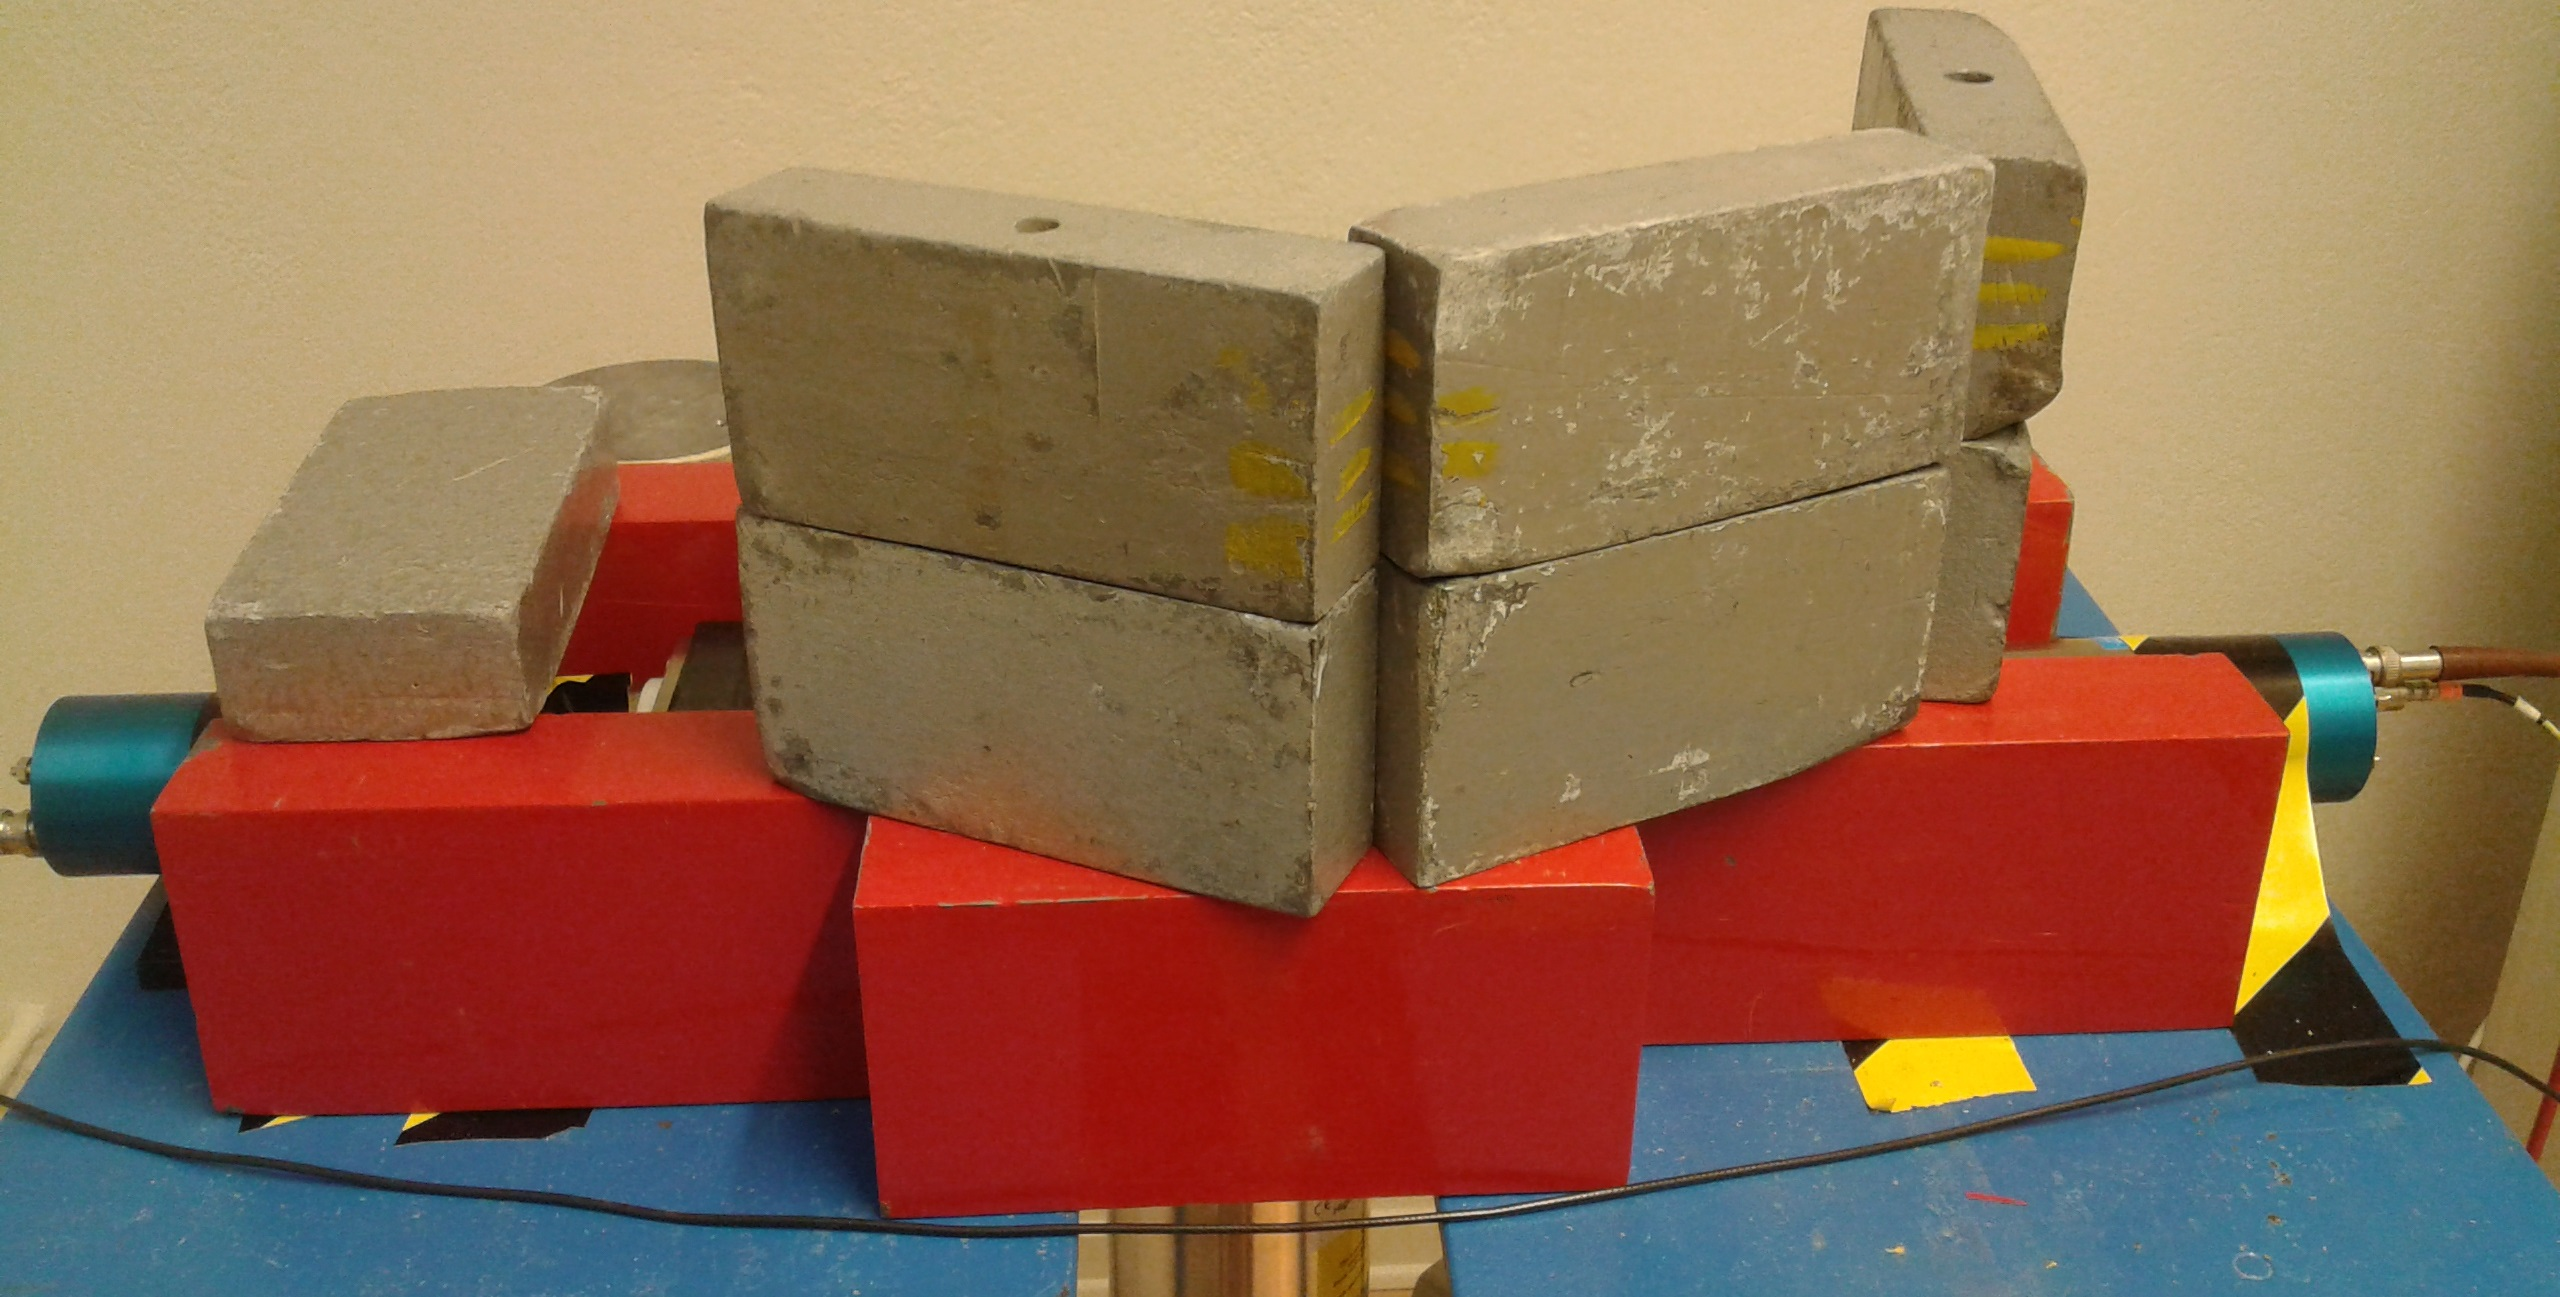
\includegraphics[scale=0.15]{New_setup_front.jpg}
\caption{Front side of the original setup (with the lead shielding). Two holed lead bricks can be seen on this picture as the one used to obtain a collimated beam.}
\label{Setup_front}
\end{figure}

\subsection{Process of measurement} \label{protocol}

For this first set of measurements, only the germanium detector was used but not the scintillator detectors. The goal of this experiment was to determine some properties of the detector depending on the location of the collimated source such as the resolution of the crystal. Therefore, the source was directed in five different places on the top of the crystal: one measurement was performed collimating the source in the center of the crystal surface, and four in the corners of the crystal surface. This was made possible by the use of a holed lead brick on top of which the source was positionned. The scanning was conducted as described below and two different cobalt sources were used, one of $^{60}$Co and one of $^{57}$Co.

In the case of $^{60}$Co, the source was held in one of the positions until the net area \footnote{In the analysis of the spectra, two areas need to be differenciated~: the total area, which gives the total number of counts between two channels, and the net area, which gives the number of counts between two channel substracted by the background.} of the studied peak (peak at $1332~keV$) contained at least 100~000 counts to match the measurement performed by the company building the detectors. The $^{57}$Co source being way less active, the measurement was stopped when the net area of the studied peak (peak at $122~keV$) contained around 1~000 counts.

The very first step was to perform the calibration. To do so, the two lines present in the spectrum of $^{60}$Co were used (lines at $1173~keV$ and $1332~keV$) and associated to a channel in the 8192 channels that the multichannel analyzer contains. In order to avoid a shift in the low energy range, the line at $122~keV$ in the spectrum of $^{57}$Co was also used. Then a linear fit was performed to get the equation of channels as a function of energy that was used in the analysis procedure later on (the data analysis is described in section~\ref{analysis}).

\subsection{Electronics}

For the first set of measurements, the scintillator detectors and the coincidence setup were not used, thus the electronics are relatively simple. The germanium detector is powered by a high voltage supply as explained in section~\ref{theory}. After going through a preamplifier, included in the cryostat, the signal is sent to an amplifier. Besides amplifying the signal, the amplifier also shapes it to a Gaussian. It is then digitized by an Analog to Digital Converter, or ADC, and a multichannel analyzer sorts the digital values which are sent to the computer that collects the data using the Maestro software. Both the high voltage supply and the amplifier are Nuclear Instrumentation Modules (NIM, a standard set of modules) and are placed in a NIM crate that provides the necessary power to their operation.

\subsection{Results and analysis} \label{analysis}

\subsubsection{First prototype}

The measurements that were conducted here had two main objectives. First, they were done in order to check the values of the principal characteristics claimed by Canberra but this first experiment was also performed to get a first idea of what one could expect with the final scanning system. This way, the detector was scanned following the protocol explained in section~\ref{protocol}.

The resolution of the detector, given by the full width at half maximum (FWHM), along with the shape of the peak, emphasized by the ratios between the full width at tenth and fiftieth maximum and the FWHM, were studied. All these results are shown in the two tables below, both for the $^{60}$Co and $^{57}$Co source (Figure~\ref{recap}). For each source, the peaks in the spectra were fitted with Gaussians and the FWHM was detuced from the fit. As the fitting program uses the FWHM to optimise the fit, the value given by the Gaussian is the same as the real value that can be read from the data. This is not the case when it comes to the FWTM and FWFM and these values were directly read on the spectra without using the fit.

\begin{figure}[!h]
\centering
\caption{Recap charts of the obtained results using the $^{60}$Co and $^{57}$Co sources. $^{60}$Co and $^{57}$Co were used for calibration to avoid possible shifts in the low energy range.}
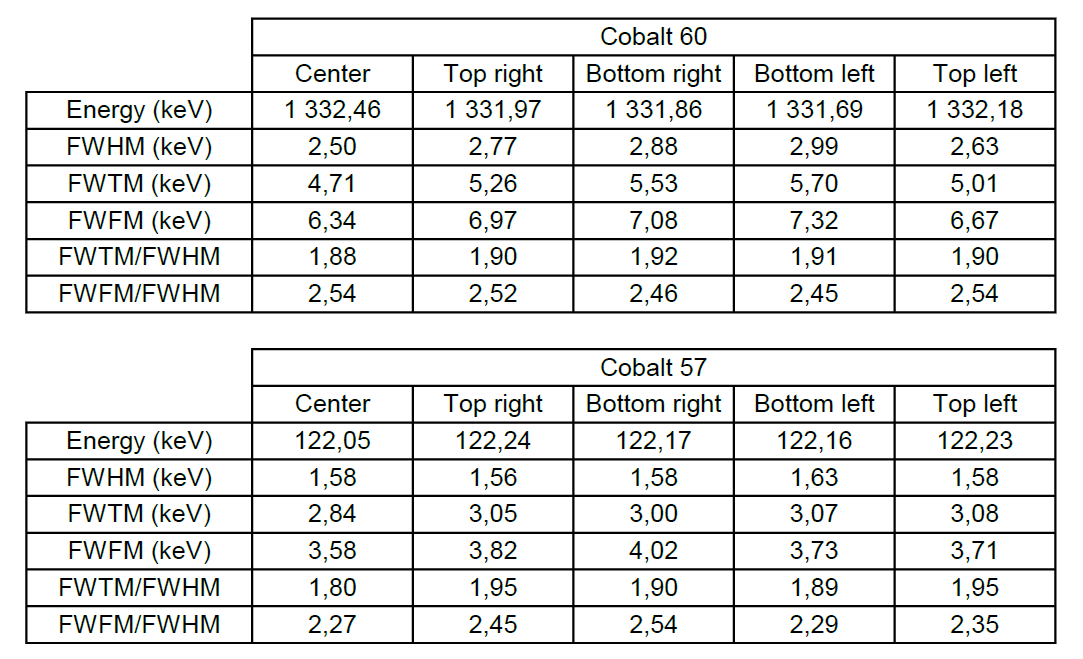
\includegraphics[scale=0.6]{Scan_Cos_2.png}
\label{recap}
\end{figure}

The very first thing we can notice in this set of measurments is that there is a shift in energy depending on where the beam was collimated. This shift in energy goes up to around $0.8~keV$ if the beam is not directed towards the center of the crystal. It is normal that the measure of the peak energy in the center of the crystal is the closest to the energy we can find in the litterature, while the calibration was made using this measurement and the measurement in the center with a $^{57}$Co source. This is also why the same measurement done in the center of the crystal with the $^{57}$Co source gives the closest result to the litterature value. The shift in energy is more important in the range of high energies and thus for the results obtained with the $^{60}$Co source. This is not an observation that is really possible to explain, but the fact that the peaks are not seen at the same energy depending on where the beam is directed is still interesting to notice. As stated in different articles treating the subject, this could come from the difference of path the charge carriers need to travel depending if the interaction happens in a corner or in the center of the crystal. Indeed, as seen before in section~\ref{theory}, the more charge carriers have to travel to reach the electrodes and be collected, the more they are susceptible of being trapped in the crystal. This can imply a shift in energy and also differences in the measure of the resolution of the crystal as explained earlier.

The same observation can be done while looking at the resolution measured in the different parts of the crystal. As for the peak energy, the difference is not huge for measurements with the $^{57}$Co source. But for the second cobalt source, the resolution varies from $2.50~keV$ up to $2.99~keV$ which is quite a big difference. Nonetheless, these values of resolution are roughly in agreement with the values provided by Canberra for the $^{60}$Co, which were, for this first prototype, of $2.40~keV$ at $1332.5~keV$. The difference between both measurements in Lund and in Canberra can be explained by the different experimental conditions in which the measurements were done. The cryostat used with the crystal could influence the measured resolution, as welle as the electronics and the treatment protocol of the data. While the first is not critical, an improvement in the electronics used can change the values of the resolution by quite a lot and as the program used to analyse the data was not the same in both cases, this could also influence the measured FWHM. The real problem here is the huge difference between the resolution obtained at Lund and at Canberra for the $^{57}$Co source~: $1.59~keV$ were measured in Lund and $0.81~keV$ which means almost twice what the final goal is. This could be explained by the $^{57}$Co source used in Lund~: the source was too weak and the net area of 100~000 counts under the peak recommended by Canberra could not be reached. These values were measured with a net area of around 1~000 counts under the peak which was thus not pointing as high over the background as it should have.

Finally, the symmetry ratios have been calculated and compared to the values given by Canberra. Again, for the $^{57}$Co source, it may not make a lot of sense to look at those values, as the peak is not large enough to be analyzed in a proper way. The values obtained for the $^{60}$Co source are closer to the theoretical values than the values given by Canberra ($1.90$ and $2.50$ against $2.19$ and $ $), indicating that the peaks obtained on the spectra have a better Gaussian shape.

\subsubsection{Second prototype}

For the second prototype, the goal was just to do the measurements to check the values provided by Canberra for this prototype and the detector was not scanned as the first prototype. Instead, the source was just placed at the exact same distance from the cap as described in~\ref{setup} but not collimated using a lead brick, in order to get a proper number of counts per second. Results are shown in chart~\ref{recap2} for the different sources that were used.

\begin{figure}[!h]
\centering
\caption{Comparative chart of the obtained resolution using, from left to right, $^{241}$Am, $^{57}$Co, $^{60}$Co and $^{137}$Cs. $^{60}$Co and $^{57}$Co were used for calibration to avoid possible shifts in the low energy range.}
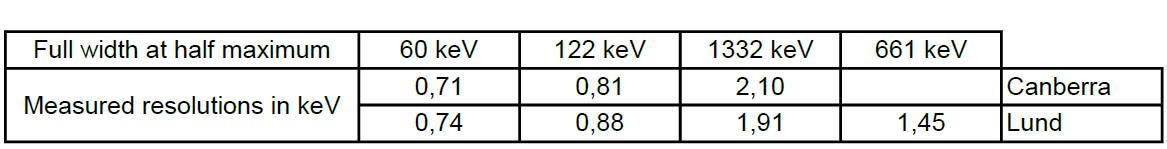
\includegraphics[scale=0.6]{result_2.png}
\label{recap2}
\end{figure}
Here the main focus was the measure of the resolution that should match the values given by Canberra (except for the cesium source, which was just performed to have a value of resolution in that range of energies). In the three cases that were given by Canberra, the results were in agreement and there was no critical measures like it was the case with the first crystal. The low energy resolution was found to be way higher than the one from the first crystal and overall the resolution increased quite significantly compared to the other detector. As for the first tested prototype, all these results are to be optimised using better electronics and cryostat as well as optimising the data analysis routine.

The shape factors of the peaks were also determined and matched quite well the ones given by the company, again slightly better than the ones from the first crystal (Figure~\ref{shape2}). The difference between these values can also be explained by the use of different electronics, that could lead to a better peak shape even if the differences are not significantly high.

\begin{figure}[!h]
\centering
\caption{Comparative chart of the peak shape at $1332.5~keV$ from the $^{60}$Co spectrum.}
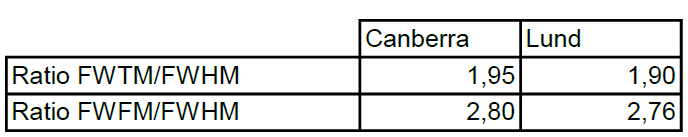
\includegraphics[scale=0.7]{shape.png}
\label{shape2}
\end{figure}
These results are quite interesting to analyse because the main difference between both crystals is the length of the hole in the middle, which is longer for the second prototype. What is important here is that the capacitance of the crystal increases with the length of the hole and thus, the resolution should decrease as the hole gets longer (see section~\ref{theory}). This is nonetheless not the case and the behaviour looks exactly the opposite, while the resolution increased with the second crystal. One of the reasons for that could be that as the length of the hole is increasing, the mean path of the charge carriers to travel to the inner electrode is decreasing and thus trapping is getting less important. As discussed earlier, effects of trapping can be really important on both the count rate and the resolution of the detector. From these results it could even be said that effects of trapping are much more important than capacitance as resolution was better for the second prototype. Trapping is also a big problem when it comes to the shape of the peak, which again confirms the fact that trapping was affected by the length of the hole and that a longer hole is better to obtain a good resolution in a semi-conductor detector. Finally, the quality of the crystal, which is not provided by the company, could highly affect the resolution of the detector and the first crystal may have been worse than the second one, also explaining the differences in resolution obtained.

\end{document}